\documentclass{beamer}
\usepackage[english]{babel}
\usepackage{color}
\usepackage{hyperref}
\usepackage{graphicx}
\usepackage[utf8x]{inputenc}
\usepackage{mhchem}
\usepackage{amsmath}
\usepackage{amssymb}
\usepackage{amsfonts}
\usepackage{amsopn}
\usepackage{braket}
\usepackage{bbm}
\usepackage{dsfont}
\usepackage{kpfonts}
% \usepackage{mathabx}

\parindent=0cm


% Various new commands that ease typesetting math even further
% \newcommand{\assign}{\ensuremath{\coloneq}}
% \newcommand{\rassign}{\ensuremath{\eqcolon}}
\newcommand{\assign}{\ensuremath{:=}}
\newcommand{\rassign}{\ensuremath{=:}}

\newcommand{\of}[1]{\ensuremath{\left( #1 \right)}}
\newcommand{\ofs}[1]{\ensuremath{\left( #1 \right)}}

\newcommand{\norm}[1]{\ensuremath{\| #1 \|}}

\newcommand{\tmop}[1]{\ensuremath{\operatorname{#1}}}

\newcommand{\id}{\ensuremath{\mathds{1}}}
% \newcommand{\id}{\ensuremath{I}}


\newcommand{\conj}[1]{\ensuremath{\overline{#1}}}

\newcommand{\T}{\ensuremath{{}^{\textnormal{T}}}}
\newcommand{\herm}{\ensuremath{{}^{\textnormal{H}}}}

\newcommand{\ft}[1]{\ensuremath{\mathcal{F}\left(#1\right)}}
\newcommand{\ift}[1]{\ensuremath{\mathcal{F}^{-1}\left(#1\right)}}

\newcommand{\fft}[1]{\ensuremath{\mathtt{FFT}\left(#1\right)}}
\newcommand{\ifft}[1]{\ensuremath{\mathtt{IFFT}\left(#1\right)}}

\newcommand{\dotp}[2]{\ensuremath{\langle #1 , #2 \rangle}}

\newcommand{\bigO}[1]{\ensuremath{\mathcal{O}\left( #1 \right)}}

\newcommand{\mat}[1]{\ensuremath{\mathbf{#1}}}

% multi-indices
\newcommand{\mindex}[1]{\ensuremath{\underline{#1}}}

\newcommand{\laplace}{\ensuremath{\operatorname{\Delta}}}

% EOF

\usepackage{graphicx}
\usepackage{subcaption}
\usepackage{asymptote}
\usepackage{tikz}
\usetikzlibrary{shapes,arrows}


\mode<presentation>
{
  \usetheme{Montpellier}
  \setbeamercovered{transparent}
}

\title[Wavepackets]{Wavepacket propagation in D-dimensional non-adiabatic crossings}
\author[]{Raoul Bourquin\\~\\ Dr. Vasile Gr\u{a}dinaru\\ Prof. Dr. Ralf Hiptmair}

\date{Seminar for Applied Mathematics, ETH Zurich \\Spring semester 2012}

\newcommand{\burl}[1]{\footnotesize{\url{#1}}}

\beamertemplatenavigationsymbolsempty
% -----------------------------------------------------------------------------------------
\begin{document}

\begin{frame}
  \titlepage
\end{frame}


\begin{frame}{Outline}
  \tableofcontents
\end{frame}


\section{Time-dependent Schrödinger equation}
\subsection{Introduction}


\begin{frame}{Time-dependent Schrödinger equation}{Semi-classical scaling}
  \begin{equation*} \label{eq:basics_tdse_semi}
    i \varepsilon^2 \frac{\partial}{\partial t} \Ket{\psi} = \underbrace{\left(\mat{T}+\mat{V}\right)}_{\mat{H}} \Ket{\psi}
  \end{equation*}
  where
  \begin{equation*}
    \mat{T} \assign - \frac{1}{2} \varepsilon^4 \Delta \qquad
    \mat{V} \assign \mat{V}\ofs{\vec{x}}
  \end{equation*}
  \begin{itemize}
  \item Time evolution for a state $\Ket{\psi(\vec{x}, t)}$
  \item Kinetic operator $\mat{T}$ and potential $\mat{V}\left(\vec{x}\right)$
  \item Semi-classical scaling $\varepsilon^2 \approx 10^{-2}, 10^{-3}, \ldots$
  \item Recover classical mechanics for $\varepsilon \rightarrow 0$
  \end{itemize}
\end{frame}


\begin{frame}{The non-adiabatic potential}
  \begin{itemize}
  \item Non-adiabatic potential $\mat{V}$ with $N$ energy levels
  \item $\mat{V}\left(\vec{x}\right)$ is a matrix dependent on $\vec{x}\in\mathbb{R}^D$
  \item \emph{Energy levels} given by the eigenvalues $\lambda_i\left(\vec{x}\right)$
  \item Levels can cross or show \emph{avoided crossings}
    \begin{itemize}
    \item There is an \emph{energy gap} $\delta$
    \end{itemize}
  \end{itemize}
  \begin{center}
    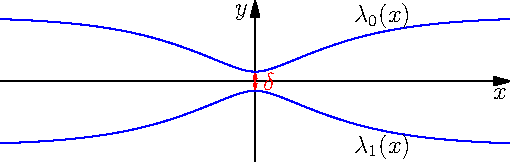
\includegraphics[scale=0.8]{./fig/potential.pdf}
  \end{center}
  % \begin{itemize}
  % \item $\Ket{\Psi}$ is a vector
  % \end{itemize}
\end{frame}


\begin{frame}{The non-adiabatic potential}{A two-dimensional example}
  \begin{equation*}
    \mat{V}(x,y) \assign
    \begin{pmatrix}
      x                   & \sqrt{y^2+\delta^2} \\
      \sqrt{y^2+\delta^2} & -x
    \end{pmatrix}
  \end{equation*}
  \begin{center}
    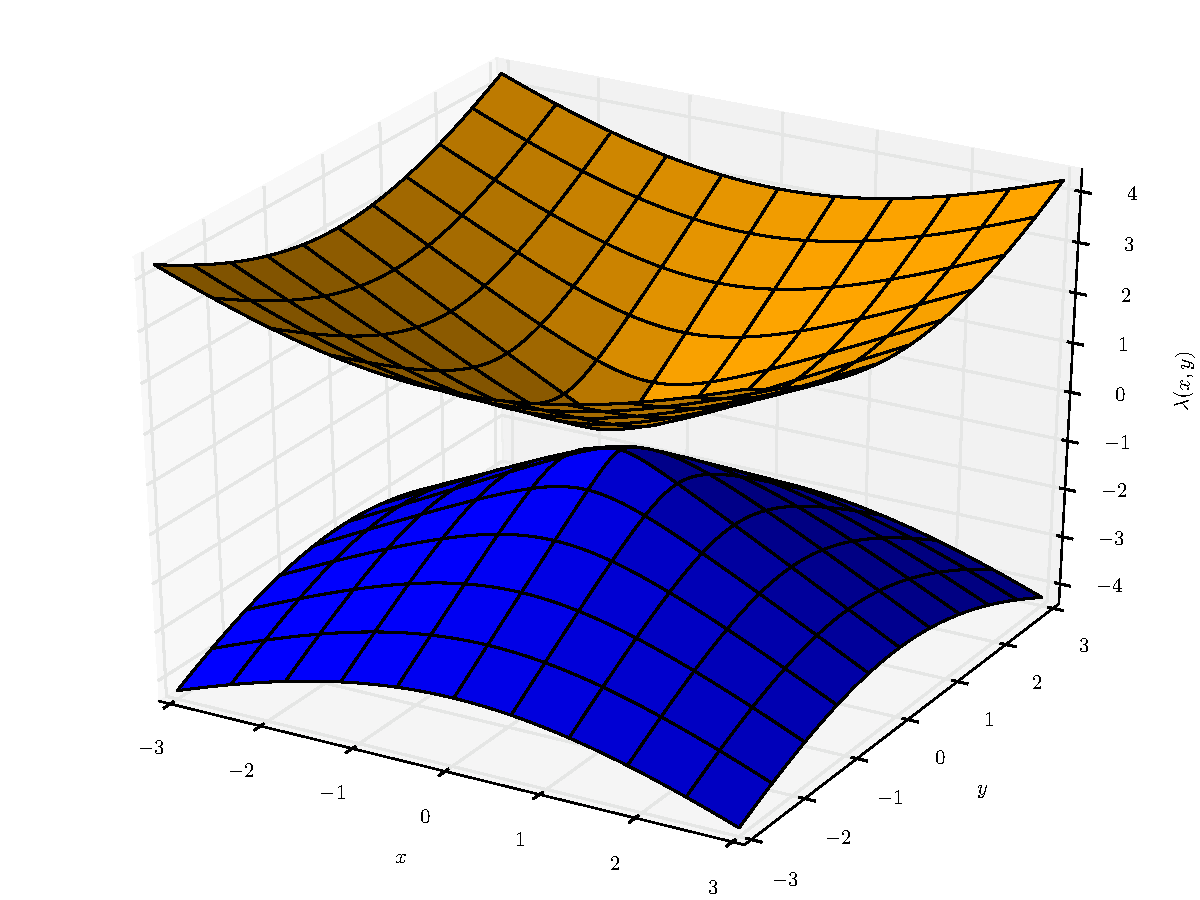
\includegraphics[scale=0.3]{./fig/conic_avoided.pdf}
  \end{center}
\end{frame}


\begin{frame}{Time-dependent Schrödinger equation}{Initial values}
  \begin{center}
    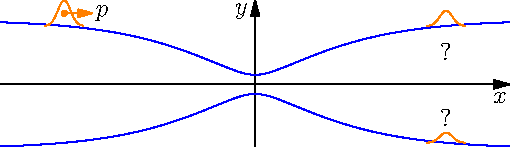
\includegraphics[scale=0.8]{./fig/iv.pdf}
  \end{center}
  \begin{itemize}
  \item Put a wavepacket $\Ket{\Psi}$ somewhere
  \item Add an initial momentum (optional)
  \item See what happens at (and after) the avoided crossing
  \item Expect some \emph{transitions}, magnitude of amplitudes?
  \end{itemize}
\end{frame}


\section{Semi-classical wavepackets}


\begin{frame}{Wavefunction}{Representation of the wavefunction}
  \begin{itemize}
  \item Separation of variables
  \item Basis set expansion
    \begin{itemize}
    \item very successful idea ($\rightarrow$ Roothaan equations in Hartree-Fock)
    \end{itemize}
  \item Parametrised basis functions
  \end{itemize}
  \begin{align*}
    \psi\ofs{\vec{x},t} & = \sum_{\vec{k}\in\mathfrak{K}} c_{\vec{k}}\ofs{t} \phi_{\vec{k}}\ofs{\vec{x}} \\
    & = \sum_{\vec{k}\in\mathfrak{K}} c_{\vec{k}}\ofs{t} \phi_{\vec{k}}\left[\Pi\ofs{t}\right]\ofs{\vec{x}}
  \end{align*}
  Parameters:
  \begin{equation*}
    \Pi\ofs{t} \assign \{\vec{q}\ofs{t}, \vec{p}\ofs{t}, \mat{Q}\ofs{t}, \mat{P}\ofs{t}\}
  \end{equation*}
  Expansion coefficients:
  \begin{equation*}
    \vec{c}\ofs{t} \assign \left\{ c_\vec{k}\ofs{t} \right\}_{\vec{k}\in\mathfrak{K}}
  \end{equation*}
\end{frame}


\begin{frame}{Semi-classical wavepackets}{Definition of the basis functions}
  \begin{itemize}
  \item Basis functions: product of a Gaussian times a polynomial
  \item Ground state
  \end{itemize}
  \begin{align*}
    \phi_{\vec{0}}[\Pi]\left(\vec{x}\right)
    \assign &
    (\pi\varepsilon^2)^{-\frac{D}{4}} (\det\mat{Q})^{-\frac{1}{2}}
    \\
    & \cdot \exp \left( \frac{i}{2\varepsilon^2}
      \dotp{(\vec{x}-\vec{q})}{\mat{P}\mat{Q}\inv(\vec{x}-\vec{q})}
      + \frac{i}{\varepsilon^2} \dotp{\vec{p}}{(\vec{x}-\vec{q})}
    \right)
  \end{align*}

  \begin{itemize}
  \item Parameters $\mat{Q} \in \mathbb{C}^{D \times D}$, $\mat{P} \in \mathbb{C}^{D \times D}$
  \item Position $\vec{q} \in \mathbb{R}^D$ and momentum $\vec{p} \in \mathbb{R}^D$
  \item Construct $\phi_\vec{k}$ by applying the \emph{raising operator} $\mathcal{R}$
  \item $\left\{\phi_{\vec{k}}\right\}_{\vec{k}}$ complete basis of $L^2$ for fixed $\Pi$
  \end{itemize}
\end{frame}


\begin{frame}{Semi-classical wavepackets}{Raising operators}
  \begin{itemize}
  \item Define the \emph{raising operator} \footnote{for details, see \cite{H_ladder_operators}}
  \end{itemize}
  \begin{equation*}
    \mathcal{R} \assign
    \begin{pmatrix}
      \mathcal{R}_0 \\
      \vdots \\
      \mathcal{R}_{D-1}
    \end{pmatrix}
    =
    \frac{i}{\sqrt{2\varepsilon^2}} \left( \mat{P}\H \left(\vec{x}-\vec{q}\right) - \mat{Q}\H \left(\left(-i \varepsilon^2 \nabla_x\right)-\vec{p}\right) \right)
  \end{equation*}
  \begin{itemize}
  \item Apply to the ground state
  \end{itemize}
  \begin{equation*}
    \phi_{\vec{k}} \assign \frac{1}{\sqrt{\vec{k}!}} \, \mathcal{R}_0^{k_0} \mathcal{R}_1^{k_1} \cdots \mathcal{R}_{D-1}^{k_{D-1}} \, \phi_{\vec{0}}
  \end{equation*}
  \begin{itemize}
  \item Higher order functions $\phi_{\vec{k}}$
  \end{itemize}
\end{frame}


\begin{frame}{Semi-classical wavepackets}{Basis function example}
  \begin{center}
    \centering
    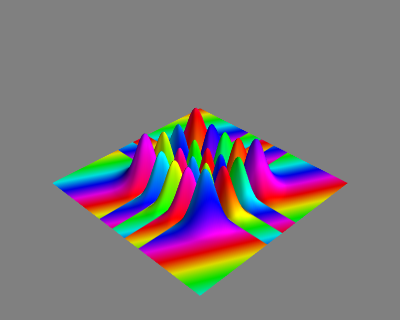
\includegraphics[scale=0.4]{./fig/phi_4-3.png}
  \end{center}
  \begin{itemize}
  \item Example of $\phi_{4,3}(x,y)$
  \end{itemize}
\end{frame}


\begin{frame}{Semi-classical wavepackets}{Basis shapes}
  \begin{itemize}
  \item \emph{Basis shapes} specify the set $\mathfrak{K}$
  \item Finite subset of $\mathbb{N}_0^D$
  \end{itemize}
  Hyperbolic cut basis shape
  \begin{minipage}{0.6\linewidth}
    \begin{equation*}
      \mathfrak{K}(K) \assign \left\{ \vec{k} \in \mathbb{N}_0^D :
        \, \prod_{d=0}^{D-1}(1+k_d) \leq K \right\}
    \end{equation*}
    \begin{itemize}
    \item Full hypercubic set grows $\mathcal{O}\left(K^D\right)$
    \item This one grows $\mathcal{O}\left(K \log(K)^{D-1}\right)$
    \end{itemize}
  \end{minipage}
  \begin{minipage}{0.29\linewidth}
    \begin{center}
      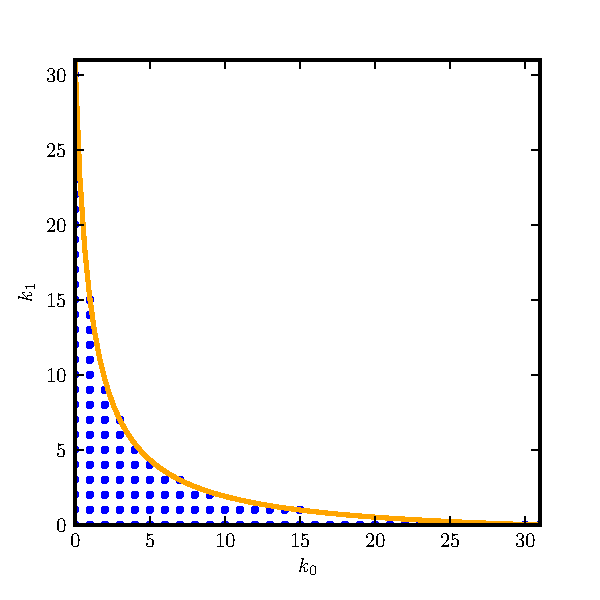
\includegraphics[scale=0.4]{./fig/hyperbolic_shape_2_32.pdf}
    \end{center}
  \end{minipage}
\end{frame}


\begin{frame}{Semi-classical wavepackets}{Definition of a wavepacket}
  \begin{itemize}
  \item General wavepacket as linear combination
  \end{itemize}
  \begin{equation*}
    \Phi\of{\vec{x}} \assign e^{\frac{iS}{\varepsilon^2}} \sum_{\vec{k}\in\mathfrak{K}} c_\vec{k} \phi_\vec{k} \of{\vec{x}}
  \end{equation*}
  \begin{itemize}
  \item In theory $\mathfrak{K} = \mathbb{N}_0^D$, practically $|\mathfrak{K}| < 200$
  \end{itemize}
  \begin{itemize}
  \item We need a vector of multiple $\Phi$
    \begin{itemize}
    \item Global parameter set $\Pi \assign \{\vec{q}, \vec{p}, \mat{Q}, \mat{P}, S\}$
    \item Individual coefficients $\left\{c_{\vec{k}}^j\right\}_\vec{k}$ per component $\Phi_j$
    \end{itemize}
  \end{itemize}
  \begin{align*} \label{eq:hawp_def_state_vector}
    \Ket{\Psi\ofs{\vec{x}}} & \assign \Ket{ \begin{pmatrix}
        \Phi_0\of{\vec{x}} \\
        \vdots \\
        \Phi_{N-1}\of{\vec{x}} \\
      \end{pmatrix}}
  \end{align*}
\end{frame}


\section{Propagation of semi-classical wavepackets}


\begin{frame}{Propagation of semi-classical wavepackets}
  \begin{itemize}
  \item Time propagation of wavepackets \footnote{generalised algorithm of \cite{FGL_semiclassical_dynamics}}
    \begin{itemize}
    \item propagate parameters $\mat{Q}$, $\mat{P}$, $\vec{q}$, $\vec{p}$ and $S$
    \item propagate all coefficients $\left\{c_{\vec{k}}\right\}_\vec{k}$
    \end{itemize}
  \item \emph{Wavepackets stay in the same mathematical form}
  \end{itemize}
\end{frame}


\begin{frame}{Theorems about exact propagation}
  Plug $\Ket{\Psi}$ into the TDSE and propagate \\~ \\
  \begin{itemize}
  \item Exact propagation only changes the values of $\Pi$
  \item We have exact propagation iff
    \begin{itemize}
    \item $H = T$
    \item $H = U$ where $U$ is quadratic
    \end{itemize}
  \item Otherwise: propagation changes the values of $\vec{c}$
    \begin{itemize}
    \item $H = W$ where $W = V - U$ is the non-quadratic remainder
    \end{itemize}
  \item Split the Schrödinger equation and propagate by $T$, $U$ and $W$ separately
  \end{itemize}
\end{frame}


\begin{frame}{Propagation of semi-classical wavepackets}{Update rules}
  \begin{itemize}
  \item Kinetic operator $T$ part
  \end{itemize}
  \begin{equation*}
    \begin{split}
      \vec{q}(t) & = \vec{q}(0) + t \,  \vec{p}(0) \\
      \mat{Q}(t) & = \mat{Q}(0) + t \,  \mat{P}(0) \\
      S(t) & = S(0) + \frac{1}{2}t \, \vec{p}(0)\T  \vec{p}(0)
    \end{split}
  \end{equation*}
  \begin{itemize}
  \item Potential part, quadratic approximation $U(\vec{x})$
  \end{itemize}
  \begin{equation*}
    \begin{split}
      \vec{p}(t) & = \vec{p}(0) - t \, \nabla U(\vec{q}(0)) \\
      \mat{P}(t) & = \mat{P}(0) - t \, \nabla^2 U(\vec{q}(0)) \mat{Q}(0) \\
      S(t) & = S(0) - t \, U(\vec{q}(0))
    \end{split}
  \end{equation*}
\end{frame}


\begin{frame}{Propagation of semi-classical wavepackets}{Galerkin approximation}
  \begin{itemize}
  \item Galerkin approximation
  \end{itemize}
  \begin{equation*}
    \forall \vec{k} \in \mathfrak{K} \quad \langle \phi_{\vec{k}}, (i\varepsilon^2\partial_t -W) u \rangle = 0
  \end{equation*}
  \begin{itemize}
  \item Non-quadratic remainder $W(\vec{x})$ part
  \end{itemize}
  \begin{equation*}
    \vec{c}(t) = \exp\left(-\frac{i}{\varepsilon^2} t \mat{F}\right) \vec{c}(0)
  \end{equation*}
  \begin{itemize}
  \item with
  \end{itemize}
  \begin{equation*}
    \mat{F} =
    \begin{pmatrix}
      {}     & \vdots                                  & {} \\
      \cdots & \dotp{\phi_{\vec{k}}}{W \phi_{\vec{l}}} & \cdots \\
      {}     & \vdots                                  & {}
    \end{pmatrix}
  \end{equation*}
\end{frame}


\subsection{Advantages of wavepackets}


\begin{frame}{Some final remarks}
  \begin{itemize}
  \item Wavepackts work very well for simpler potentials
  \item Some open issues for more complex potentials
    \begin{itemize}
    \item Several parameters to choose, for example the basis size
    \end{itemize}
  \end{itemize}
  \begin{itemize}
  \item Gridless method
    \begin{itemize}
    \item but we need very high order quadrature
    \item and the matrix exponential of a full matrix
      \begin{itemize}
      \item Iterative methods like Arnoldi
      \end{itemize}
    \end{itemize}
  \end{itemize}
  \begin{itemize}
  \item Unbounded domains possible
  \end{itemize}
\end{frame}


\section{Examples}


\begin{frame}{A simulation example}{Missed conic crossing}
  \begin{itemize}
  \item Take the potential \\
    \begin{minipage}{0.6\linewidth}
      \begin{equation*}
        \mat{V}(x,y) \assign
        \begin{pmatrix}
          x                   & \sqrt{y^2+\delta^2} \\
          \sqrt{y^2+\delta^2} & -x
        \end{pmatrix}
      \end{equation*}
    \end{minipage}
    \begin{minipage}{0.29\linewidth}
      \begin{center}
        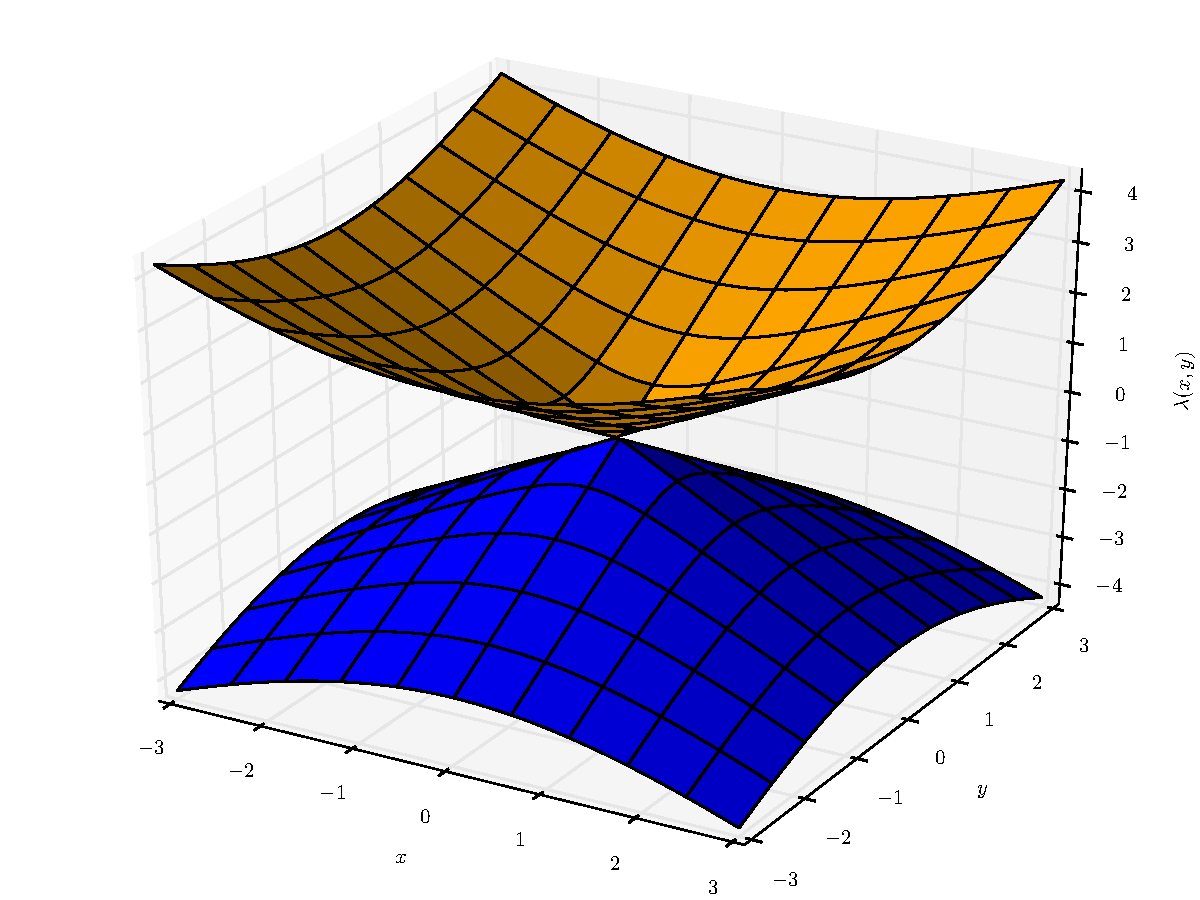
\includegraphics[scale=0.15]{./fig/conic_intersection.pdf}
      \end{center}
    \end{minipage}
  \item Set $\delta = 0$ and $\varepsilon = 0.01$
  \item Initial parameters $\Pi$
    \begin{align*}
      \vec{q} = \begin{pmatrix}
        -0.1 \\ \alpha \varepsilon
      \end{pmatrix}
      \quad
      \vec{p} = \begin{pmatrix}
        1 \\ 0
      \end{pmatrix}
      \quad
      \mat{Q} = \begin{pmatrix}
        1 & 0 \\ 0 & 1
      \end{pmatrix}
      \quad
      \mat{P} = \begin{pmatrix}
        i & 0 \\ 0 & i
      \end{pmatrix}
      \quad
      S = 0
    \end{align*}
  \item Timestep $\tau = 0.001$
  \item Start with a Gaussian $\phi_{\vec{0}}$
  \item Vary $\alpha$
  \end{itemize}
\end{frame}


\begin{frame}{A simulation example}{Missed conic crossing, $\alpha = 1.0$}
  \begin{figure}
    \centering
    \subfloat[][]{
      \label{fig:mca_16_1-0_0-01_e}
      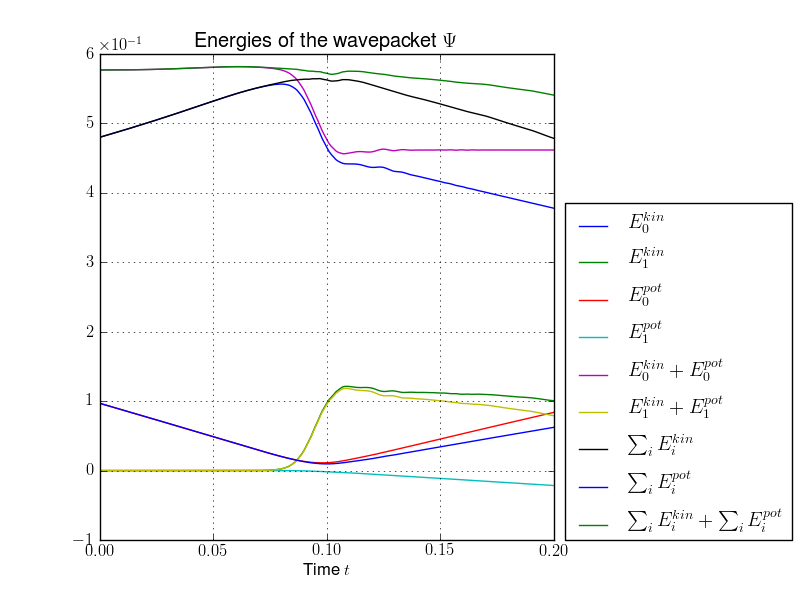
\includegraphics[width=0.5\linewidth]{./results/Parameters[bsize=16][alpha=1-0][eps=0-01]/energies_block0.png}
    }
    \subfloat[][]{
      \label{fig:mca_16_1-0_0-01_n}
      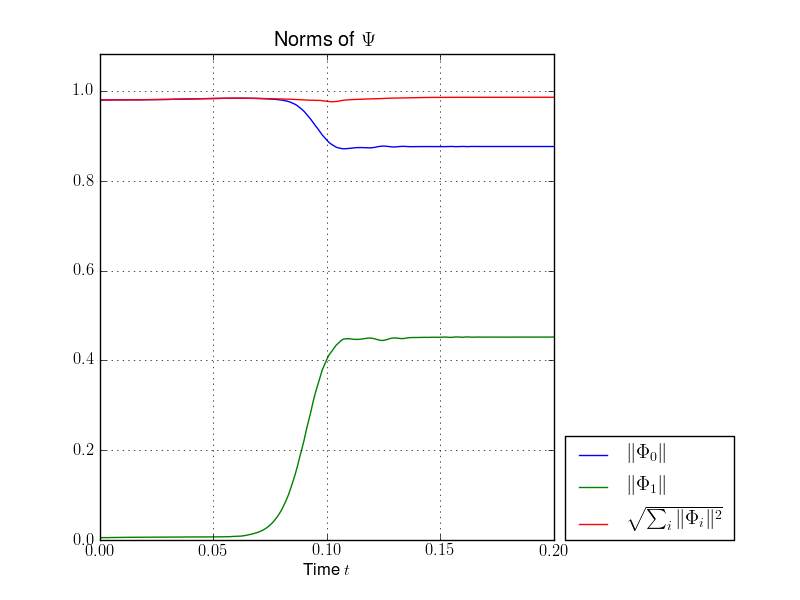
\includegraphics[width=0.5\linewidth]{./results/Parameters[bsize=16][alpha=1-0][eps=0-01]/norms_block0.png}
    }
  \end{figure}
\end{frame}


\begin{frame}{A simulation example}{Missed conic crossing, $\alpha = 1.5$}
  \begin{figure}
    \centering
    \subfloat[][]{
      \label{fig:mca_16_1-5_0-01_e}
      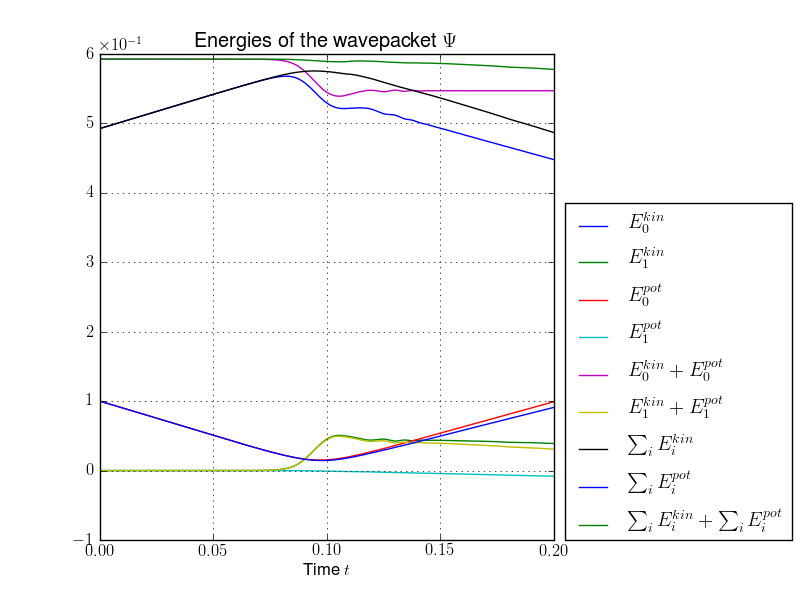
\includegraphics[width=0.5\linewidth]{./results/Parameters[bsize=16][alpha=1-5][eps=0-01]/energies_block0.png}
    }
    \subfloat[][]{
      \label{fig:mca_16_1-5_0-01_n}
      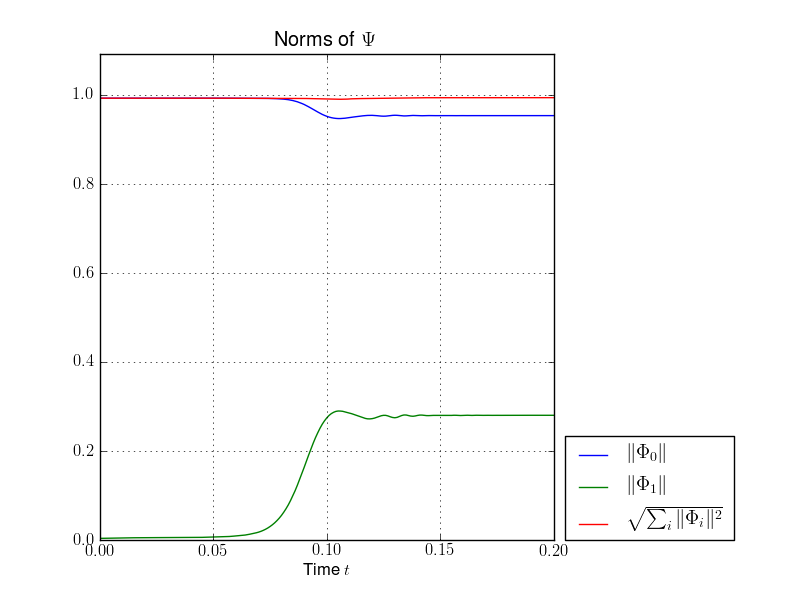
\includegraphics[width=0.5\linewidth]{./results/Parameters[bsize=16][alpha=1-5][eps=0-01]/norms_block0.png}
    }
  \end{figure}
\end{frame}


\begin{frame}{A simulation example}{Missed conic crossing, $\alpha = 2.0$}
  \begin{figure}
    \centering
    \subfloat[][]{
      \label{fig:mca_16_2-0_0-01_e}
      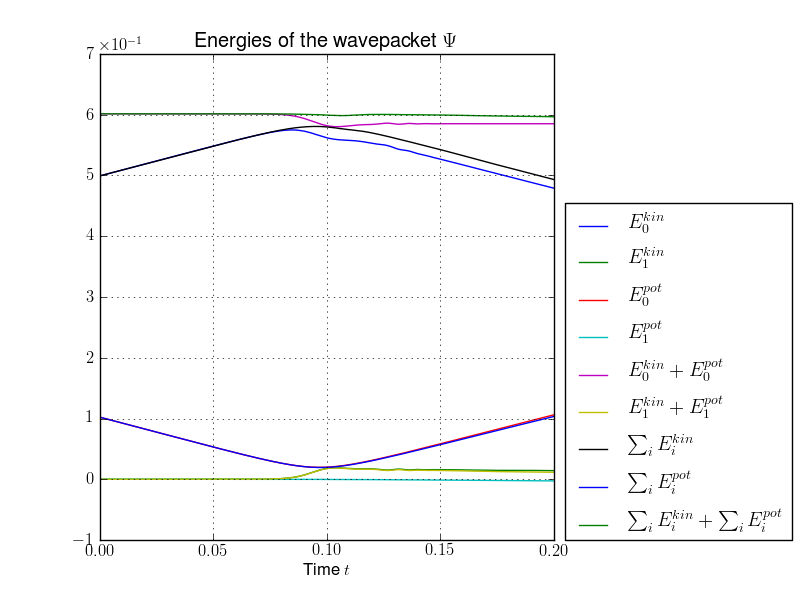
\includegraphics[width=0.5\linewidth]{./results/Parameters[bsize=16][alpha=2-0][eps=0-01]/energies_block0.png}
    }
    \subfloat[][]{
      \label{fig:mca_16_2-0_0-01_n}
      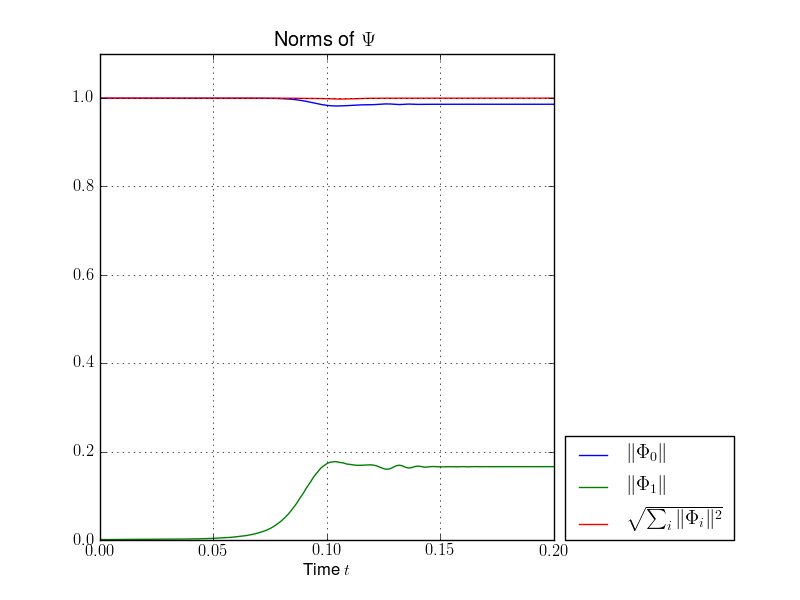
\includegraphics[width=0.5\linewidth]{./results/Parameters[bsize=16][alpha=2-0][eps=0-01]/norms_block0.png}
    }
  \end{figure}
\end{frame}


\begin{frame}{Another simulation example}{An avoided crossing}
  \begin{itemize}
  \item Take the potential \\
    \begin{minipage}{0.6\linewidth}
      \begin{equation*}
        \mat{V}(x,y) \assign
        \begin{pmatrix}
          \frac{1}{2} \xi & \delta \\
          \delta          & - \frac{1}{2} \xi
        \end{pmatrix}
      \end{equation*}
      where $\xi \assign \tanh{\left(\sqrt{x^2 + y^2} \right)}$
    \end{minipage}
    \begin{minipage}{0.3\linewidth}
      \begin{center}
        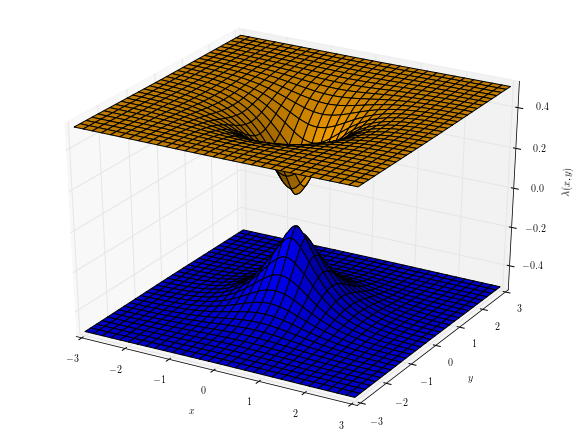
\includegraphics[scale=0.15]{./fig/delta_gap_rotsym.png}
      \end{center}
    \end{minipage}
  \item Initial parameters $\Pi$
    \begin{align*}
      \vec{q} = \begin{pmatrix}
        -3 \\ 0
      \end{pmatrix}
      \quad
      \vec{p} = \begin{pmatrix}
        0.5 \\ 0
      \end{pmatrix}
      \quad
      \mat{Q} = \begin{pmatrix}
        1 & 0 \\ 0 & 1
      \end{pmatrix}
      \quad
      \mat{P} = \begin{pmatrix}
        i & 0 \\ 0 & i
      \end{pmatrix}
      \quad
      S = 0
    \end{align*}
  \item Timestep $\tau = 0.01$
  \item Start with a Gaussian $\phi_{\vec{0}}$
  \item Vary $\varepsilon$ and $\delta$
  \end{itemize}
\end{frame}


\begin{frame}{Another simulation example}{An avoided crossing with $\varepsilon=0.01$ and $\delta=0.05$}
  \begin{figure}
    \centering
    \subfloat[][]{
      \label{fig:mca_16_2-0_0-01_e}
      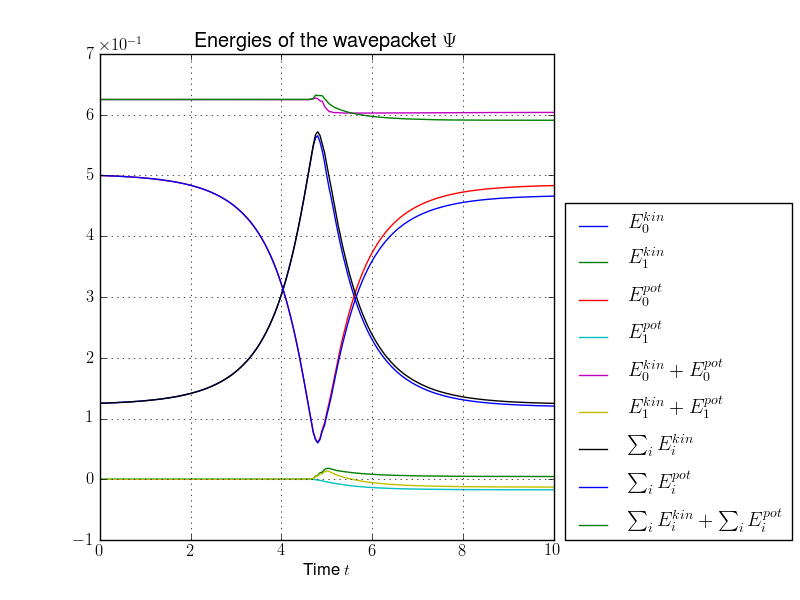
\includegraphics[width=0.5\linewidth]{./results/Parameters[bsize=16][eps=0-01][delta=0-05]/energies_block0.png}
    }
    \subfloat[][]{
      \label{fig:mca_16_2-0_0-01_n}
      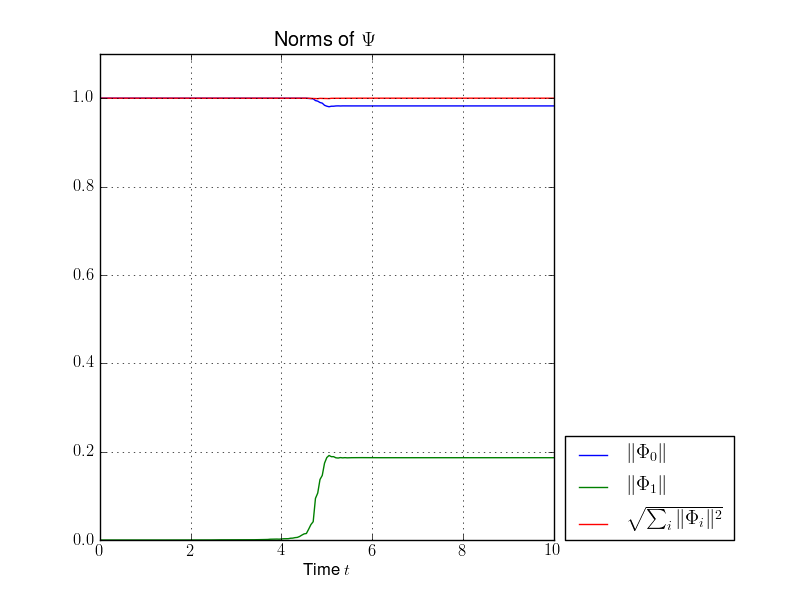
\includegraphics[width=0.5\linewidth]{./results/Parameters[bsize=16][eps=0-01][delta=0-05]/norms_block0.png}
    }
  \end{figure}
\end{frame}


\begin{frame}{Another simulation example}{An avoided crossing with $\varepsilon=0.01$ and $\delta=0.5$}
  \begin{figure}
    \centering
    \subfloat[][]{
      \label{fig:mca_16_2-0_0-01_e}
      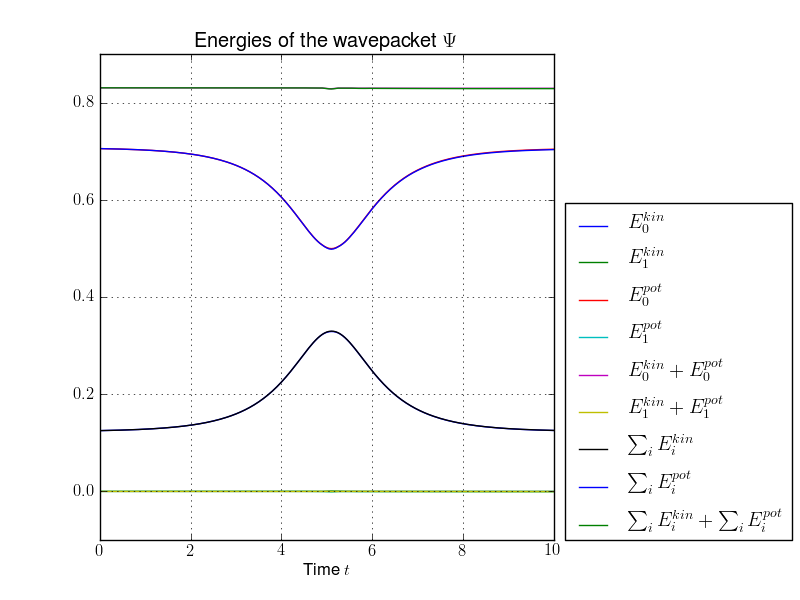
\includegraphics[width=0.5\linewidth]{./results/Parameters[bsize=16][eps=0-01][delta=0-5]/energies_block0.png}
    }
    \subfloat[][]{
      \label{fig:mca_16_2-0_0-01_n}
      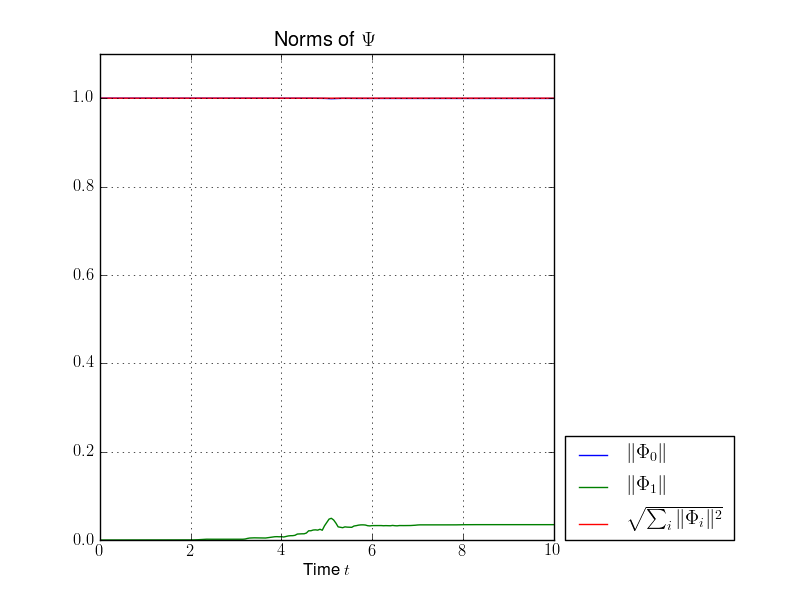
\includegraphics[width=0.5\linewidth]{./results/Parameters[bsize=16][eps=0-01][delta=0-5]/norms_block0.png}
    }
  \end{figure}
\end{frame}


\section{Current and future work}


\begin{frame}{Current and future work}{Some ideas}
  \begin{itemize}
  \item Apply the algorithms to real chemical problems
    \begin{itemize}
    \item For example Pyrazine (\ce{C_4H_4N_2}), see \cite{Lasser}
    \item or Methyl iodide (\ce{ICH_3}), see \cite{lee_heller}
    \end{itemize}
  \end{itemize}
  \begin{itemize}
  \item Use code to simulate
    \begin{itemize}
    \item In even higher dimensions $D > 3$
    \item More than 2 energy levels
    \end{itemize}
  \end{itemize}
  \begin{itemize}
  \item Improve propagation for very small $\varepsilon$
  \end{itemize}
\end{frame}


\section{End}


\begin{frame}{Thanks for your attention}
  More information on the topic
  \begin{itemize}
  \item The full thesis:\\
    {\burl{http://www.sam.math.ethz.ch/~raoulb/research/master_thesis/tex/main.pdf}}
    % \item The python source code:\\
    %   {\burl{https://github.com/raoulbq/WaveBlocksND}}
  \end{itemize}

  \scriptsize
  \bibliographystyle{abbrv}
  \bibliography{mt,chem,wp,own}
\end{frame}

\end{document}
